\chapter{Pythagorean Triples}

\section{The Pythagorean Theorem}

Recall that a right triangle is a triangle in which one of the angles is a right angle, i.e., it is exactly $90^\circ$. The Pythagorean theorem relates the lengths of the sides of a right triangle to the length of its hypotenuse. There are many ways to prove this theorem. We will present the \emph{Chinese proof}, \emph{Euclid's proof}, and the trigonometric proof of Ne'Kiya Jackson and Calcea Johnson, who made headlines in 2023 as high school students with their remarkable discovery of a trigonometric proof \cite{theguardian2023}.

\begin{theorem}\label{theorem:pythagorean-theorem}
  Consider a right triangle with side lengths $a$ and $b$, and a hypotenuse of length $c$. Then
  \begin{equation*}
    a^2 + b^2 = c^2.
  \end{equation*}
\end{theorem}

\begin{proof}[The Chinese proof]
  Consider a square with side lengths $a+b$, and include four right triangles with side lengths $a$ and $b$ in the square, so that their right angles coincide with the four right angles of the square.
\begin{center}
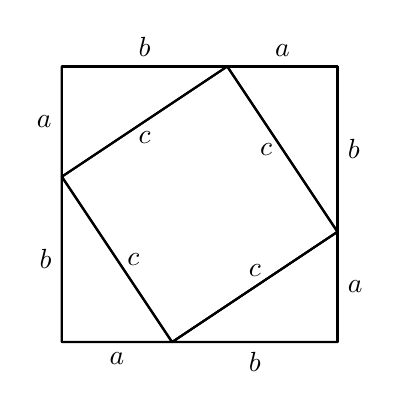
\begin{tikzpicture}[scale=.7,thick,line join=round]
    % Define points of the outer square
    \coordinate (A) at (0,0);
    \coordinate (B) at (5,0);
    \coordinate (C) at (5,5);
    \coordinate (D) at (0,5);
    
    % Define points of the inner square
    \coordinate (E) at (2,0);
    \coordinate (F) at (5,2);
    \coordinate (G) at (3,5);
    \coordinate (H) at (0,3);
    
    % Draw the outer square
    \draw[thick] (A) -- (B) -- (C) -- (D) -- cycle;
    
    % Draw the four right triangles
    \draw (A) -- node[below] {$a$} (E) -- (H) -- node[left] {$b$} cycle;
    \draw (E) -- node[below] {$b$} (B) -- node[right] {$a$} (F) -- cycle;
    \draw (F) -- node[right] {$b$} (C) -- node[above] {$a$} (G) -- cycle;
    \draw (G) -- node[above] {$b$} (D) -- node[left] {$a$} (H) -- cycle;
    
    % Draw the inner square
    \draw[line join=bevel] (E) -- node[midway,above] {$c$} (F) -- node[midway,left] {$c$} (G) -- node[midway,below] {$c$} (H) -- node[midway,right] {$c$} cycle;
\end{tikzpicture}
\end{center}
  The area of the square is $(a+b)^2$. On the other hand, the area of each triangle is $ab/2$. Combined with the area of the inner square, whose sides are the hypotenuses of the four triangles, we obtain that
  \begin{equation*}
    (a+b)^2 = c^2 + 4\frac{ab}{2} = c^2 + 2ab.
  \end{equation*}
  Since $(a+b)^2=a^2+2ab+b^2$, we find that $a^2+b^2=c^2$.
\end{proof}

\begin{proof}[Euclid's proof]
  Consider a right triangle $ACB$ with hypotenuse $AB$, and draw a line from $C$ through $AB$ at a right angle. The intersection point is called $M$.
  \begin{equation*}
    \begin{tikzpicture}[scale=.1,line join=round,line cap=round]
      \pgfmathsetmacro{\myangle}{atan(28/45)}
      \pgfmathsetmacro{\CM}{28*45/53}
      
      \coordinate (A) at (0,0);
      \coordinate (B) at (53,0);
      \coordinate (C) at ($(A) + ({90-\myangle}:28)$);
      \coordinate (M) at ($(C) + (270:\CM)$);
      
      \draw[thick] (A) -- (C) -- (B) -- cycle;
      \draw[thick] (C) -- (M);
      
      \draw (M) ++(0:2) -- ++(90:2) -- ++(180:2);
      
      \node[below left]  at (A) {$A$};
      \node[below right] at (B) {$B$};
      \node[above]       at (C) {$C$};
      \node[below right] at (M) {$M$};
      
      \draw pic[draw=black, angle radius=10] {angle=B--A--C};
      \draw pic[draw=black, angle radius=10] {angle=M--C--B};
      
      \path (B) -- (C) node[midway, above right] {$a$};
      \path (A) -- (C) node[midway, above left] {$b$};
      
      % Add a brace for the entire segment AB
      \draw[decorate, decoration={brace, amplitude=3pt, mirror}]
      ($(A)+(0,-5)$) -- ($(B)+(0,-5)$) node[midway, yshift=-3mm] {$c$};
    \end{tikzpicture}
  \end{equation*}
  Let $x$ be the length of the line segment $AM$, and let $y$ be the length of the line segment $BM$, so that $x+y=c$. The line $CM$ divides the triangle $ACB$ into two triangles $CMA$ and $CMB$, both of which are similar to the original triangle $ACB$. Thus, the ratio $a:c$ is the same as the ratio $y:a$, and the ratio $b:c$ is the same as the ratio $x:b$. This gives us the equalities
  \begin{equation*}
    a^2 = cy\qquad\text{and}\qquad b^2 = cx.
  \end{equation*}
  Since $x+y=c$, we find that $a^2+b^2=c^2$.
\end{proof}

Our third proof and final proof in this section, which is due to Ne'Kiya Jackson and Calcea Johnson, is remarkable because it makes essential use of trigonometric functions sine and cosine and the addition law, which can be derived trigonometrically, rather than on calculations involving areas of shapes. Besides its use of trigonometry, it is remarkable because Ne'Kiya Jackson and Calcea Johnson were still in high school when they found their proof, and it stands out for its inventive creativity.

\begin{wrapfigure}{r}{.4\textwidth}
  \centering
  \begin{tikzpicture}[scale=.7,line join=round,line cap=round]
    % Draw the triangle
    \coordinate (A) at (0,0);
    \coordinate (B) at (4,3);
    \coordinate (C) at (4,0);
    
    \draw[thick] (A) -- (C) node[midway, below] {$\cos(\theta)$} -- (B) node[midway, right] {$\sin(\theta)$} -- cycle node[midway, above] {$1$};
    
    % Mark right angle
    \draw (4,0) -- ++(-0.4,0) -- ++(0,0.4) -- ++(0.4,0);

    \draw pic[draw=black, angle radius=15,"$\theta$" {xshift=13,yshift=4}] {angle=C--A--B};

    \node[above right] at (B) {$B$};
    \node[below left] at (A) {$A$};
    \node[below right] at (C) {$C$};
  \end{tikzpicture}
\end{wrapfigure}
Recall that the sine and cosine functions are defined to be the lengths of the vertical and horizontal sides of a right triangle, as indicated in the diagram on the side.

This means that if $ABC$ is a right triangle with side $BC$ of length $a$, side $AC$ of length $b$, hypotenuse $AB$ of length $c$, and angle $\theta:=\angle CAB$, then we have
\begin{equation*}
  \sin(\theta) = \frac{a}{c}\qquad\text{and}\qquad \cos(\theta)=\frac{b}{c}.
\end{equation*}
In the proof of the Pythagorean theorem, we will make use of the addition formulas for sine and cosine:
\begin{align*}
  \sin(\theta + \phi) & = \sin(\theta)\cos(\phi) + \cos(\theta)\sin(\phi) \\
  \cos(\theta + \phi) & = \sin(\theta)\sin(\phi) - \cos(\theta)\cos(\phi).
\end{align*}
In particular, $\sin(2\theta)=2\sin(\theta)\cos(\theta)$, and $\cos(2\theta)=\sin^2(\theta)-\cos^2(\theta)$. These laws can be derived geometrically if $\theta+\phi$ is an acute angle, i.e., if it is strictly less than $90^\circ$, see \cref{exercise:addition-laws-sin-cos}.

\begin{proof}[The Jackson--Johnson proof \cite{jacksonjohnson2024}]
  Consider a right triangle $ABC$ with the right angle at $C$, and label the sides $a=BC$, $b=AC$, and $c=AB$ so $c$ is the hypotenuse.

  In the special case where $ABC$ is isosceles, i.e., if $a=b$, the hypotenuse is the diagonal of an $a$-by-$a$ square, which gives us that $c^2=2a^2$. Hence, we may assume that $ABC$ is nonisosceles.

  Without loss of generality, we will assume that $a<b$, i.e., that $BC$ is the shorter side. We reflect the triangle along the longer side $AC$, as indicated in the diagram below:
  \begin{equation*}
    \begin{tikzpicture}[scale=.2,line join=round,line cap=round]
      \pgfmathsetmacro{\length}{((2 * (64 / 225)) / (1 - (64 / 225)))}

      \coordinate (B) at (0,0);
      \coordinate (C) at (8,0);
      \coordinate (B') at (16,0);
      \coordinate (A) at (8,15);

      \node[below left] at (B) {$B$};
      \node[above] at (A) {$A$};
      \node[below] at (C) {$C$};
      \node[below right] at (B') {$B'$};      

      \draw[thick] (B) -- (C) -- (B') -- (A) -- cycle;
      \draw[thick] (A) -- (C);

      \path (B) -- (C) node[midway, below] {$a$};
      \path (B) -- (A) node[midway, above left] {$c$};
      \path (B') -- (C) node[midway, below] {$a$};
      \path (A) -- (B') node[midway, above right] {$c$};
      \path (A) -- (C) node[pos=0.66,left] {$b$};
      
      \draw pic[draw=black, angle radius=15,"$\theta$" {xshift=-3,yshift=-13}] {angle=B--A--C};
      \draw pic[draw=black, angle radius=15,"$\theta$" {xshift=3,yshift=-13}] {angle=C--A--B'};

    \end{tikzpicture}
  \end{equation*}

  Observe that the angle $\theta := \angle BAC$ is strictly less than $45^\circ$, so that the angle $2\theta = \angle BAB'$ is still an acute angle.

  Using this combined triangle, we draw a line from $B$ perpendicular to the line $AB$, and we extend the line $AB'$ until they meet in an intersection point, which we call $D$. This construction yields a new right triangle $ABD$ with the right angle at $B$, as in \cref{figure:jackson-johnson-pythagorean-theorem}.
  \begin{figure}[t]
    \centering
    \begin{tikzpicture}[scale=.2,line join=round,line cap=round]
      \pgfmathsetmacro{\length}{((2 * (64 / 225)) / (1 - (64 / 225)))}

      \coordinate (B) at (0,0);
      \coordinate (C) at (8,0);
      \coordinate (B') at (16,0);
      \coordinate (A) at (8,15);
      \coordinate (D) at ($ (B')!\length!180:(A)$);

      \node[left] at (B) {$B$};
      \node[right] at (B') {$B'$};
      \node[above] at (A) {$A$};
      \node[below right] at (D) {$D$};      


      \draw[thick,gray,dashed] (B') -- (A) -- (B);
      \draw[thick,gray,dashed] (A) -- (C);
      \draw[thick] (B) -- (C) -- (B') -- (D) -- cycle;

      \draw[thick] (B') -- (D);
      \draw[thick] (D) -- (B);

      \draw pic [draw=black, angle radius=3mm] {right angle=A--B--D};

      \draw[thick,line join=bevel]
      (B') -- ++(0,{-16 * (8/15)}) coordinate (E)
      -- ++({16 * (8/15)^2},0) coordinate (F)
      -- ++(0,{-16 * (8/15)^3}) coordinate (G)
      -- ++({16 * (8/15)^4},0) coordinate (H)
      -- ++(0,{-16 * (8/15)^5})
      -- ++({16 * (8/15)^6},0)
      -- ++(0,{-16 * (8/15)^7});

      \node[below left] at (E) {$E$};
      \node[above right] at (F) {$F$};
      \node[below left] at (G) {$G$};
      \node[above right] at (H) {$H$};

      \draw pic[draw=black, angle radius=18] {angle=B--A--C};
      \draw pic[draw=black, angle radius=18,"$\theta$" {xshift=13,yshift=-3}] {angle=D--B--C};
      \draw pic[draw=black, angle radius=13] {angle=E--B'--D};
      \draw pic[draw=black, angle radius=10] {angle=D--E--F};
    \end{tikzpicture}
    \caption[A diagram in the Jackson--Johnson proof]{The recursive subdivision of the triangle $BDB'$.}
    \label{figure:jackson-johnson-pythagorean-theorem}
  \end{figure}

  We will now subdivide the triangle $BDB'$ by first dropping a line down from $B'$ at a right angle from the line $BB'$, creating a new right triangle $BEB'$. Since this triangle also has an angle $\theta$, it is similar to the original triangle $ABC$. Its sides have lengths $2a$ and $2a^2/b$.

  We continue subdividing the triangle $BDB'$ into ever smaller right triangles, as indicated in the figure. The successive triangles in this sequence are all right triangles with an angle $\theta$, so they are all similar. Corresponding sides in these successive triangles have a ratio of $a/b$. The hypotenuses of these triangles therefore have length
  \begin{equation*}
    2c\left(\frac{a}{b}\right)^n
  \end{equation*}
  This allows us to calculate the length of the side $B'D$ via the formula for the geometric series, which we proved in \cref{theorem:formula-geometric-series}:
  \begin{equation*}
    |B'D| = \sum_{k=0}^\infty 2c\left(\frac{a}{b}\right)^{2k+2} = 2c\left(\frac{a}{b}\right)^2\sum_{k=0}^\infty \left(\frac{a}{b}\right)^{2k} = \frac{2c\left(\frac{a}{b}\right)^2}{1-\left(\frac{a}{b}\right)^2}=\frac{2ca^2}{b^2-a^2}.
  \end{equation*}
  Now we can find two expressions for the length of the line $AD$. First, it consists of the lines $AB'$ and $B'D$, so it is of length $c+|B'D|$, which we calculated above. On the other hand, by trigonometry we have that $c/|AD|=\cos(2\theta)$, which gives us that $|AD|=c/\cos(2\theta)$. Since both expressions give the length of the line $AD$, both involving a factor of $c$ which we can factor out, we obtain the following equation:
  \begin{equation*}
    1+\frac{2a^2}{b^2-a^2} = \frac{1}{\cos(2\theta)}.
  \end{equation*}
  Furthermore, the addition formula for cosines gives us that $\cos(2\theta)=\sin^2(\theta)-\cos^2(\theta)$. Since $\sin(\theta)=\frac{b}{c}$ and $\cos(\theta)=\frac{a}{c}$, we find that
  \begin{equation*}
    1+\frac{2a^2}{b^2-a^2} = \frac{c^2}{b^2-a^2}.
  \end{equation*}
  Rearranging this equation gives us that $(b^2 - a^2)+2a^2 = c^2$, which yields
  \begin{equation*}
    a^2+b^2=c^2.\qedhere
  \end{equation*}
\end{proof}

\section{Euclid's Parametrization of the Pythagorean Triples}

Our goal in this section is to describe all the solutions of the quadratic Diophantine equation
\begin{equation*}
  x^2 + y^2 = z^2,
\end{equation*}
where $z$ is a nonzero integer. By the \crefnamed{theorem:pythagorean-theorem}{Pythagorean Theorem}, any such triple $(x,y,z)$ describes the lengths of the sides and hypotenuse of a right triangle. Such a triple is therefore called a \emph{Pythagorean triple}. Notice that if $(x,y,z)$ is a Pythagorean triple, then so is $(kx,ky,kz)$, and their corresponding triangles are of the same shape. Such Pythagorean triples are therefore called \emph{similar}, and we are interested in the Pythagorean triples up to similarity.

\begin{wrapfigure}{r}{.4\textwidth}
  \centering
  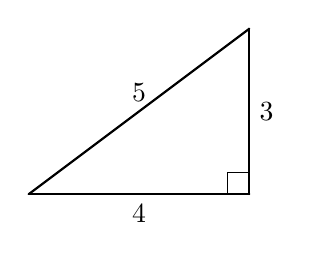
\begin{tikzpicture}[scale=.7,line join=round,line cap=round]
    % Draw the triangle
    \draw[thick] (0,0) -- (4,0) node[midway, below] {$4$};
    \draw[thick] (4,0) -- (4,3) node[midway, right] {$3$};
    \draw[thick] (4,3) -- (0,0) node[midway, above] {$5$};
    
    % Mark right angle
    \draw (4,0) -- ++(-0.4,0) -- ++(0,0.4) -- ++(0.4,0);
  \end{tikzpicture}
\end{wrapfigure}
The trivial solutions are $(0,1,1)$ and $(1,0,1)$. The simplest nontrivial solution is the famous equation
\begin{equation*}
  3^2 + 4^2 = 5^2.
\end{equation*}

\begin{figure}[t]
  \centering
  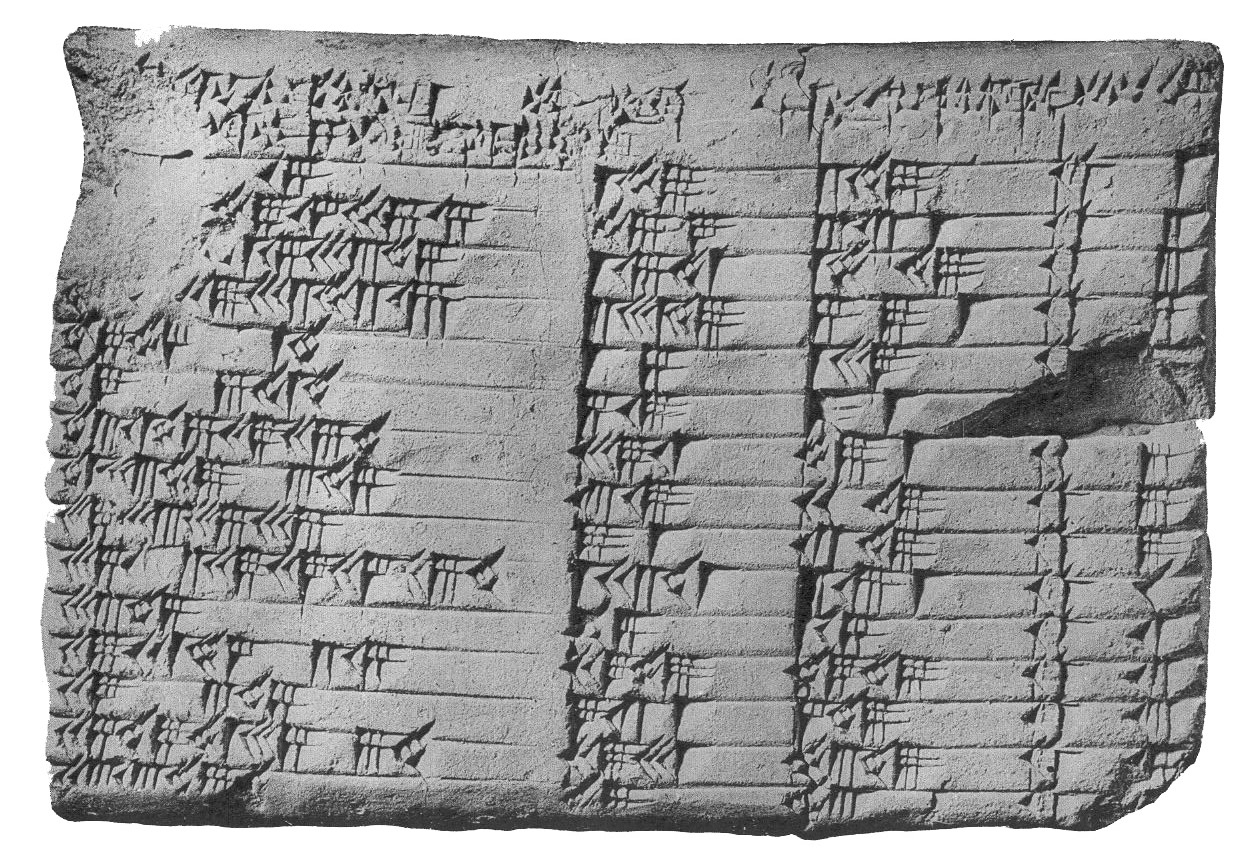
\includegraphics[width=0.68\textwidth]{Plimpton_322.jpg}
  \caption[The Babylonian tablet Plimpton 322]{The Babylonian tablet Plimpton 322, listing Pythagorean triples. }
  \label{fig:plimpton322}
\end{figure}
The triangle with side lengths $3$ and $4$ and a hypotenuse of length $5$ is sometimes called the \emph{Egyptian triangle}, since it is believed that the ancient Egyptians used this triangle for practical applications. The oldest surviving table of Pythagorean triples was created by the Babylonians, in what is now known as the tablet \emph{Plimpton 322}. This clay tablet, which is estimated to date from 1800 BCE, contains a mathematical table written in cuneiform script, where each row describes a Pythagorean triple in sexagesimal notation, i.e., base 60.

Some further Pythagorean triples include
\begin{equation*}
  (5,12,13),\qquad (21,20,29),\qquad\text{and}\qquad (15,8,17).
\end{equation*}

Fibonacci devised in his book \emph{Liber Quadratorum (The Book of Squares)} \cite{fibonacci1987} a clever way to quickly show that there are infinitely many Pythagorean triples. If an odd square $a^2$ is the $n$th odd number, i.e., if $a^2=2n+1$, then there are positive integers $b$ and $c$ such that
\begin{equation*}
  b^2 = \sum_{i=0}^{n-1}(2i+1),\qquad\text{and}\qquad c^2=\sum_{i=0}^{n}(2i+1)
\end{equation*}
by \cref{exercise:sum-of-odd-numbers}. For this choice of $a$, $b$, and $c$, we have
\begin{equation*}
  a^2 + b^2 = c^2.
\end{equation*}

\begin{proposition}
  There are infinitely many Pythagorean triples $(a,b,c)$ such that $c=b+1$.
\end{proposition}

Note that while Fibonacci used the sum of odd numbers to find a triple $(a,b,c)$ of integers such that $a^2+b^2=c^2$, these Fibonacci triples follow the pattern
\begin{equation*}
  (2b + 1) + b^2 = (b+1)^2.
\end{equation*}
Here we immediately see that if $2b+1$ is a square number $a^2$, and indeed any odd square is of this form, then we obtain a Pythagorean triple of the form $(a,b,b+1)$. Rewriting $a=2k+1$, we see that Fibonacci's Pythagorean triples are of the form
\begin{equation*}
  (2k+1,\,2k^2 + 2k,\,2k^2 + 2k+1).
\end{equation*}

The Pythagorean triples $(a,b,c)$ generated by Fibonacci's method always satisfy $c=b+1$. However, we have already seen that $(21,20,29)$ is a Pythagorean triple that is not of this form. Therefore we see that, even though Fibonacci's method can be used to see that there are infinitely many Pythagorean triples, it does not generate all of them.

In the remainder of this section we will derive the classic formula that describes all the Pythagorean triples. The method leading to this formula was described by Euclid in Book X, Proposition 29 and Book 6, Proposition 21 of the Elements.

\begin{definition}
  A \emph{primitive Pythagorean triple} is a triple $(x,y,z)$ satisfying
  \begin{equation*}
    x^2 + y^2 = z^2
  \end{equation*}
  such that $\gcd(x,y)=1$.
\end{definition}

\begin{example}
  All the Pythagorean triples generated by Fibonacci's method are primitive, since $\gcd(2b+1,b)=1$.
\end{example}

\begin{lemma}
  For any Pythagorean triple $(x,y,z)$ there is a unique primitive Pythagorean triple $(x',y',z')$ consisting of positive integers for which there is an integer $k$ such that $(kx',ky',kz')=(x,y,z)$.
\end{lemma}

\begin{proof}
  Given a Pythagorean triple $(x,y,z)$, let $k:=\gcd(x,y)$. Since $k\mid x$ and $k\mid y$, it follows from the equation $x^2+y^2=z^2$ that $k\mid z$. Thus, we define
  \begin{equation*}
    x' := x/k, \qquad y' := y/k, \qquad\text{and}\qquad z' := z/k.
  \end{equation*}
  Then $x'$ and $y'$ are relatively prime, and we have
  \begin{equation*}
    x'^2 + y'^2 = \frac{x^2+y^2}{k^2} = \frac{z^2}{k^2} = z'^2.
  \end{equation*}
  The triple $(x',y',z')$ is therefore a primitive Pythagorean triple such that
  \begin{equation*}
    (kx',ky',kz') = (x,y,z).
  \end{equation*}
  For uniqueness, suppose that $(x'',y'',z'')$ is an other such primitive Pythagorean triple, satisfying $(lx'',ly'',lz'')=(x,y,z)$. Since $\gcd(x'',y'')=1$, it follows that
  \begin{equation*}
    k=\gcd(x,y)=\gcd(lx'',ly'')=l
  \end{equation*}
  Furthermore, since at least one of $x$ or $y$ is nonzero, it follows both $k$ and $l$ are nonzero. Thus we get $x'=x''$ from the equation $kx'=kx''$, and we get $y'=y''$ from the equation $ky'=ky''$. We conclude that $(x',y',z')=(x'',y'',z'')$.
\end{proof}

By the previous lemma we can restrict our attention to primitive Pythagorean triples. Next, we do a parity analysis of the components of a primitive Pythagorean triple to show that exactly one of the components of $(x,y,z)$ in a Pythagorean triple is divisible by $4$. In \cref{exercise:divisibility-legs-pythagorean-triples} we make the similar claims that exactly one of the components of a Pythagorean triple is divisible by $3$, and exactly one divisible by $5$.

\begin{lemma}
  Consider a primitive Pythagorean triple $(x,y,z)$. Then $z$ is odd, exactly one of $x$ and $y$ is divisible by $4$, and the other is odd.
\end{lemma}

\begin{proof}
  Since $(x,y,z)$ is a primitive Pythagorean triple, it is clearly impossible for both $x$ and $y$ to be even. It is also impossible for both of them to be odd, since in that case $z^2$ would be of the form $4k+2$, which is impossible since every square is of the form $4k$ or $4k+1$. Thus, one of $x$ and $y$ is even and the other is odd. This gives us that $z^2$ is odd, which is only possible if $z$ is odd.

  It remains to show that the even component among $x$ and $y$ is in fact divisible by $4$. To this end, recall that every square is of the form $8k$, $8k+1$, or $8k+4$. Since $x^2+y^2=z^2$ is of the form $8k+1$, it is impossible for one of the squares $x^2$ or $y^2$ to be of the form $8k+4$. It follows that the even square is of the form $8k$. If $x^2$ is divisible by $8$, then clearly $x$ is divisible by $4$, and likewise if $y^2$ is divisible by $8$ then $y$ is divisible by $4$.
\end{proof}

By the previous lemma we may assume, without loss of generality, that in a primitive Pythagorean triple $(x,y,z)$, the integer $x$ is odd and the integer $y$ is even. Under this assumption, we can show that $z-x$ and $z+x$ double a square, which leads us directly to Euclid's parametrization of the Pythagorean triples.

\begin{lemma}\label{lemma:euclids-parametrization}
  Consider a primitive Pythagorean triple $(x,y,z)$ in which $y$ is even, so that $x$ is odd. Then there are two relatively prime positive integers $s<t$ of opposite parity, such that
  \begin{equation*}
    z-x=2s^2 \qquad\text{and}\qquad z+x=2t^2.
  \end{equation*}
\end{lemma}

\begin{proof}
  By the assumption that $y$ is even, we can write $y=2u$. Then we have
  \begin{equation*}
    (z-x)(z+x) = z^2-x^2 = y^2 = 4u^2.
  \end{equation*}
  Any common divisor $d$ of $z-x$ and $z+x$ must divide their sum $2z$ and their difference $2x$. However, since $x$ and $z$ are relatively prime, it follows that $d\mid 2$. On the other hand, since both $x$ and $z$ are odd it follows that $z\pm x$ is even, which implies that $d=2$. Thus we see that
  \begin{equation*}
    \left(\frac{z-x}{2}\right)\left(\frac{z+x}{2}\right)=u^2
  \end{equation*}
  is a decomposition of a square into relatively prime factors. This implies that each factor is itself a square. More precisely, there are two relatively prime positive integers $s<t$ such that
  \begin{equation*}
    \frac{z-x}{2}=s^2\qquad\text{and}\qquad\frac{z+x}{2}=t^2.
  \end{equation*}
  Furthermore, observe that since $z$ and $x$ are both odd, it follows that one of $z-x$ and $z+x$ is divisible by $4$ and the other is of the form $4k+2$. This implies that one of $s$ and $t$ is even and the other is odd.
\end{proof}

\begin{theorem}[Euclid’s Parametrization of the Pythagorean Triples]\label{theorem:euclids-parametrization}
  For every primitive Pythagorean triple $(x,y,z)$ with $y$ even, we can uniquely determine two relatively prime positive integers $s<t$ of opposite parity such that
  \begin{equation*}
    x=t^2-s^2,\qquad y=2st,\qquad\text{and}\qquad z=t^2+s^2.
  \end{equation*}
\end{theorem}

\begin{proof}
  To prove that two relatively prime integers $0<s<t$ exist as specified, we will use $s$ and $t$ as determined in \cref{lemma:euclids-parametrization}, where
  \begin{equation*}
    \frac{z-x}{2}=s^2,\qquad\text{and}\qquad\frac{z+x}{2}=t^2.
  \end{equation*}
  A simple calculation shows that $t^2-s^2=x$, and $t^2+s^2=z$. To see that $y=2st$, it suffices to show that $y^2=4s^2t^2$. This follows from the following short calculation:
  \begin{equation*}
    4s^2t^2=(z-x)(z+x)=z^2-x^2=y^2.
  \end{equation*}

  In order to show that $s$ and $t$ are uniquely determined as specified, consider additionally two relatively prime positive integers $u<v$ of opposite parity such that
    \begin{equation*}
    x=v^2-u^2,\qquad y=2uv,\qquad\text{and}\qquad z=v^2+u^2.
  \end{equation*}
  then $z-x=2u^2$ and $z+x=2v^2$, while at the same time we have $z-x=2s^2$ and $z+x=2t^2$. This implies $s^2=u^2$ and $t^2=v^2$. Since all the numbers involved are positive, we obtain that $s=u$ and $t=v$.
\end{proof}

\section{Rational Points on the Unit Circle}

The unit circle consists of all points $(u,v)$ that are a unit distance from the origin. In other words, a point $(u,v)$ in the plane with real number coordinates lies on the unit circle if it satisfies the condition
\begin{equation*}
  u^2+v^2=1.
\end{equation*}
Every Pythagorean triple $(x,y,z)$ corresponds to a point
\begin{equation*}
  \left(\frac{x}{z},\frac{y}{z}\right)
\end{equation*}
on the unit circle. Since both coordinates of the point $(\frac{x}{z},\frac{y}{z})$ are rational numbers, we say that this point is a \emph{rational point} on the unit circle.

\begin{figure}[t]
  \begin{center}
    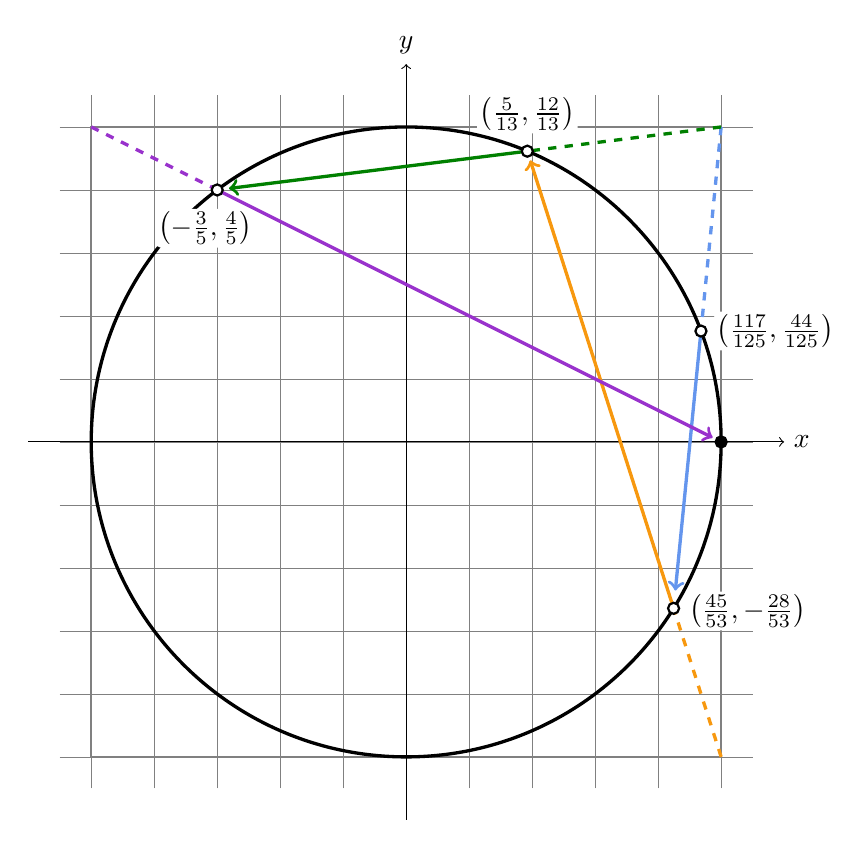
\begin{tikzpicture}[scale=4]
      % Draw the grid with spacing 0.2, extending 0.1 beyond the square
      \draw[gray,very thin] (-1.1,-1.1) grid[step=0.2] (1.1,1.1);
      
      % Draw the thick black square
      \draw[thick,Gray] (-1,-1) rectangle (1,1);
      
      % Draw the thick black circle
      \draw[very thick] (0,0) circle (1);
      
      % Draw the x and y axes as arrows
      \draw[->] (-1.2,0) -- (1.2,0) node[right] {\(x\)};
      \draw[->] (0,-1.2) -- (0,1.2) node[above] {\(y\)};
      
      % Coordinates for the node
      \coordinate (P1) at ({117/125},{44/125});
      \coordinate (P2) at ({45/53},{-28/53});
      \coordinate (P3) at ({5/13},{12/13});
      \coordinate (P4) at ({-3/5},{4/5});
    
      
      % Draw the line from (1,1) through the node
      \draw[CornflowerBlue,very thick,dashed] (1,1) -- (P1);
      \draw[CornflowerBlue,very thick,->,shorten >=1.5ex] (P1) -- (P2);
      \draw[YellowOrange,very thick,dashed] (1,-1) -- (P2);
      \draw[YellowOrange,very thick,->,shorten >=0.8ex] (P2) -- (P3);
      \draw[Green,very thick,dashed] (1,1) -- (P3);
      \draw[Green,very thick,->,shorten >=1ex] (P3) -- (P4);
      \draw[DarkOrchid,very thick,dashed] (-1,1) -- (P4);
      \draw[DarkOrchid,very thick,->,shorten >=0.8ex] (P4) -- (1,0);
      
      % Draw the node
      \draw[fill=white,thick] (P1) circle (.5pt) node[rounded corners=2pt,right,fill=white, inner sep=1pt,xshift=1ex] {\(\left(\frac{117}{125}, \frac{44}{125}\right)\)};
      \draw[fill=white,thick] (P2) circle (.5pt) node[rounded corners=2pt,right,fill=white, inner sep=1pt,xshift=1ex,yshift=-1pt] {\(\left(\frac{45}{53},-\frac{28}{53}\right)\)};
      \draw[fill=white,thick] (P3) circle (.5pt) node[rounded corners=2pt,above,fill=white, inner sep=1pt,yshift=1.4ex] {\(\left(\frac{5}{13},\frac{12}{13}\right)\)}; 
      \draw[fill=white,thick] (P4) circle (.5pt) node[rounded corners=2pt,below,fill=white, inner sep=1pt,yshift=-1.5ex,xshift=-1ex] {\(\left(-\frac{3}{5},\frac{4}{5}\right)\)};
      \draw[fill=black,thick] (1,0) circle (.5pt);
      
    \end{tikzpicture}
  \end{center}
  \caption[Vieta jumps between rational points on the unit circle]{For any rational point $(x,y)$ on the unit circle apart from $(0,\pm1)$ and $(\pm1,0)$, draw a straight line through it from the outer corner of its quadrant to find a new rational point $(x',y')$ on the unit circle. The common denominator of $(x',y')$ is strictly smaller than that of $(x,y)$, so that this process eventually terminates at $(0,\pm1)$ or $(\pm1,0)$.}
\end{figure}

\section{The Tree of Primitive Pythagorean Triples}

The set of all primitive Pythagorean triples has the structure of a rooted ternary tree. This structure was first discovered by Berggren in 1934 \cite{berggren1934}.

\begin{equation*}
  A =
  \left(
    \begin{matrix}
      1 & -2 & 2 \\
      2 & -1 & 2 \\
      2 & -2 & 3
    \end{matrix}
  \right),\qquad
  B =
  \left(
    \begin{matrix}
      1 & 2 & 2 \\
      2 & 1 & 2 \\
      2 & 2 & 3
    \end{matrix}
  \right),\qquad\text{and}\qquad
  C =
  \left(
    \begin{matrix}
      -1 & 2 & 2 \\
      -2 & 1 & 2 \\
      -2 & 2 & 3
    \end{matrix}
  \right)
\end{equation*}

\section{Squares in Arithmetic Progressions}

\begin{wrapfigure}[16]{r}{0.4\textwidth}
  \centering
  \begin{tikzpicture}
    \node[inner sep=0pt, rounded corners=0.2em, clip] {%
      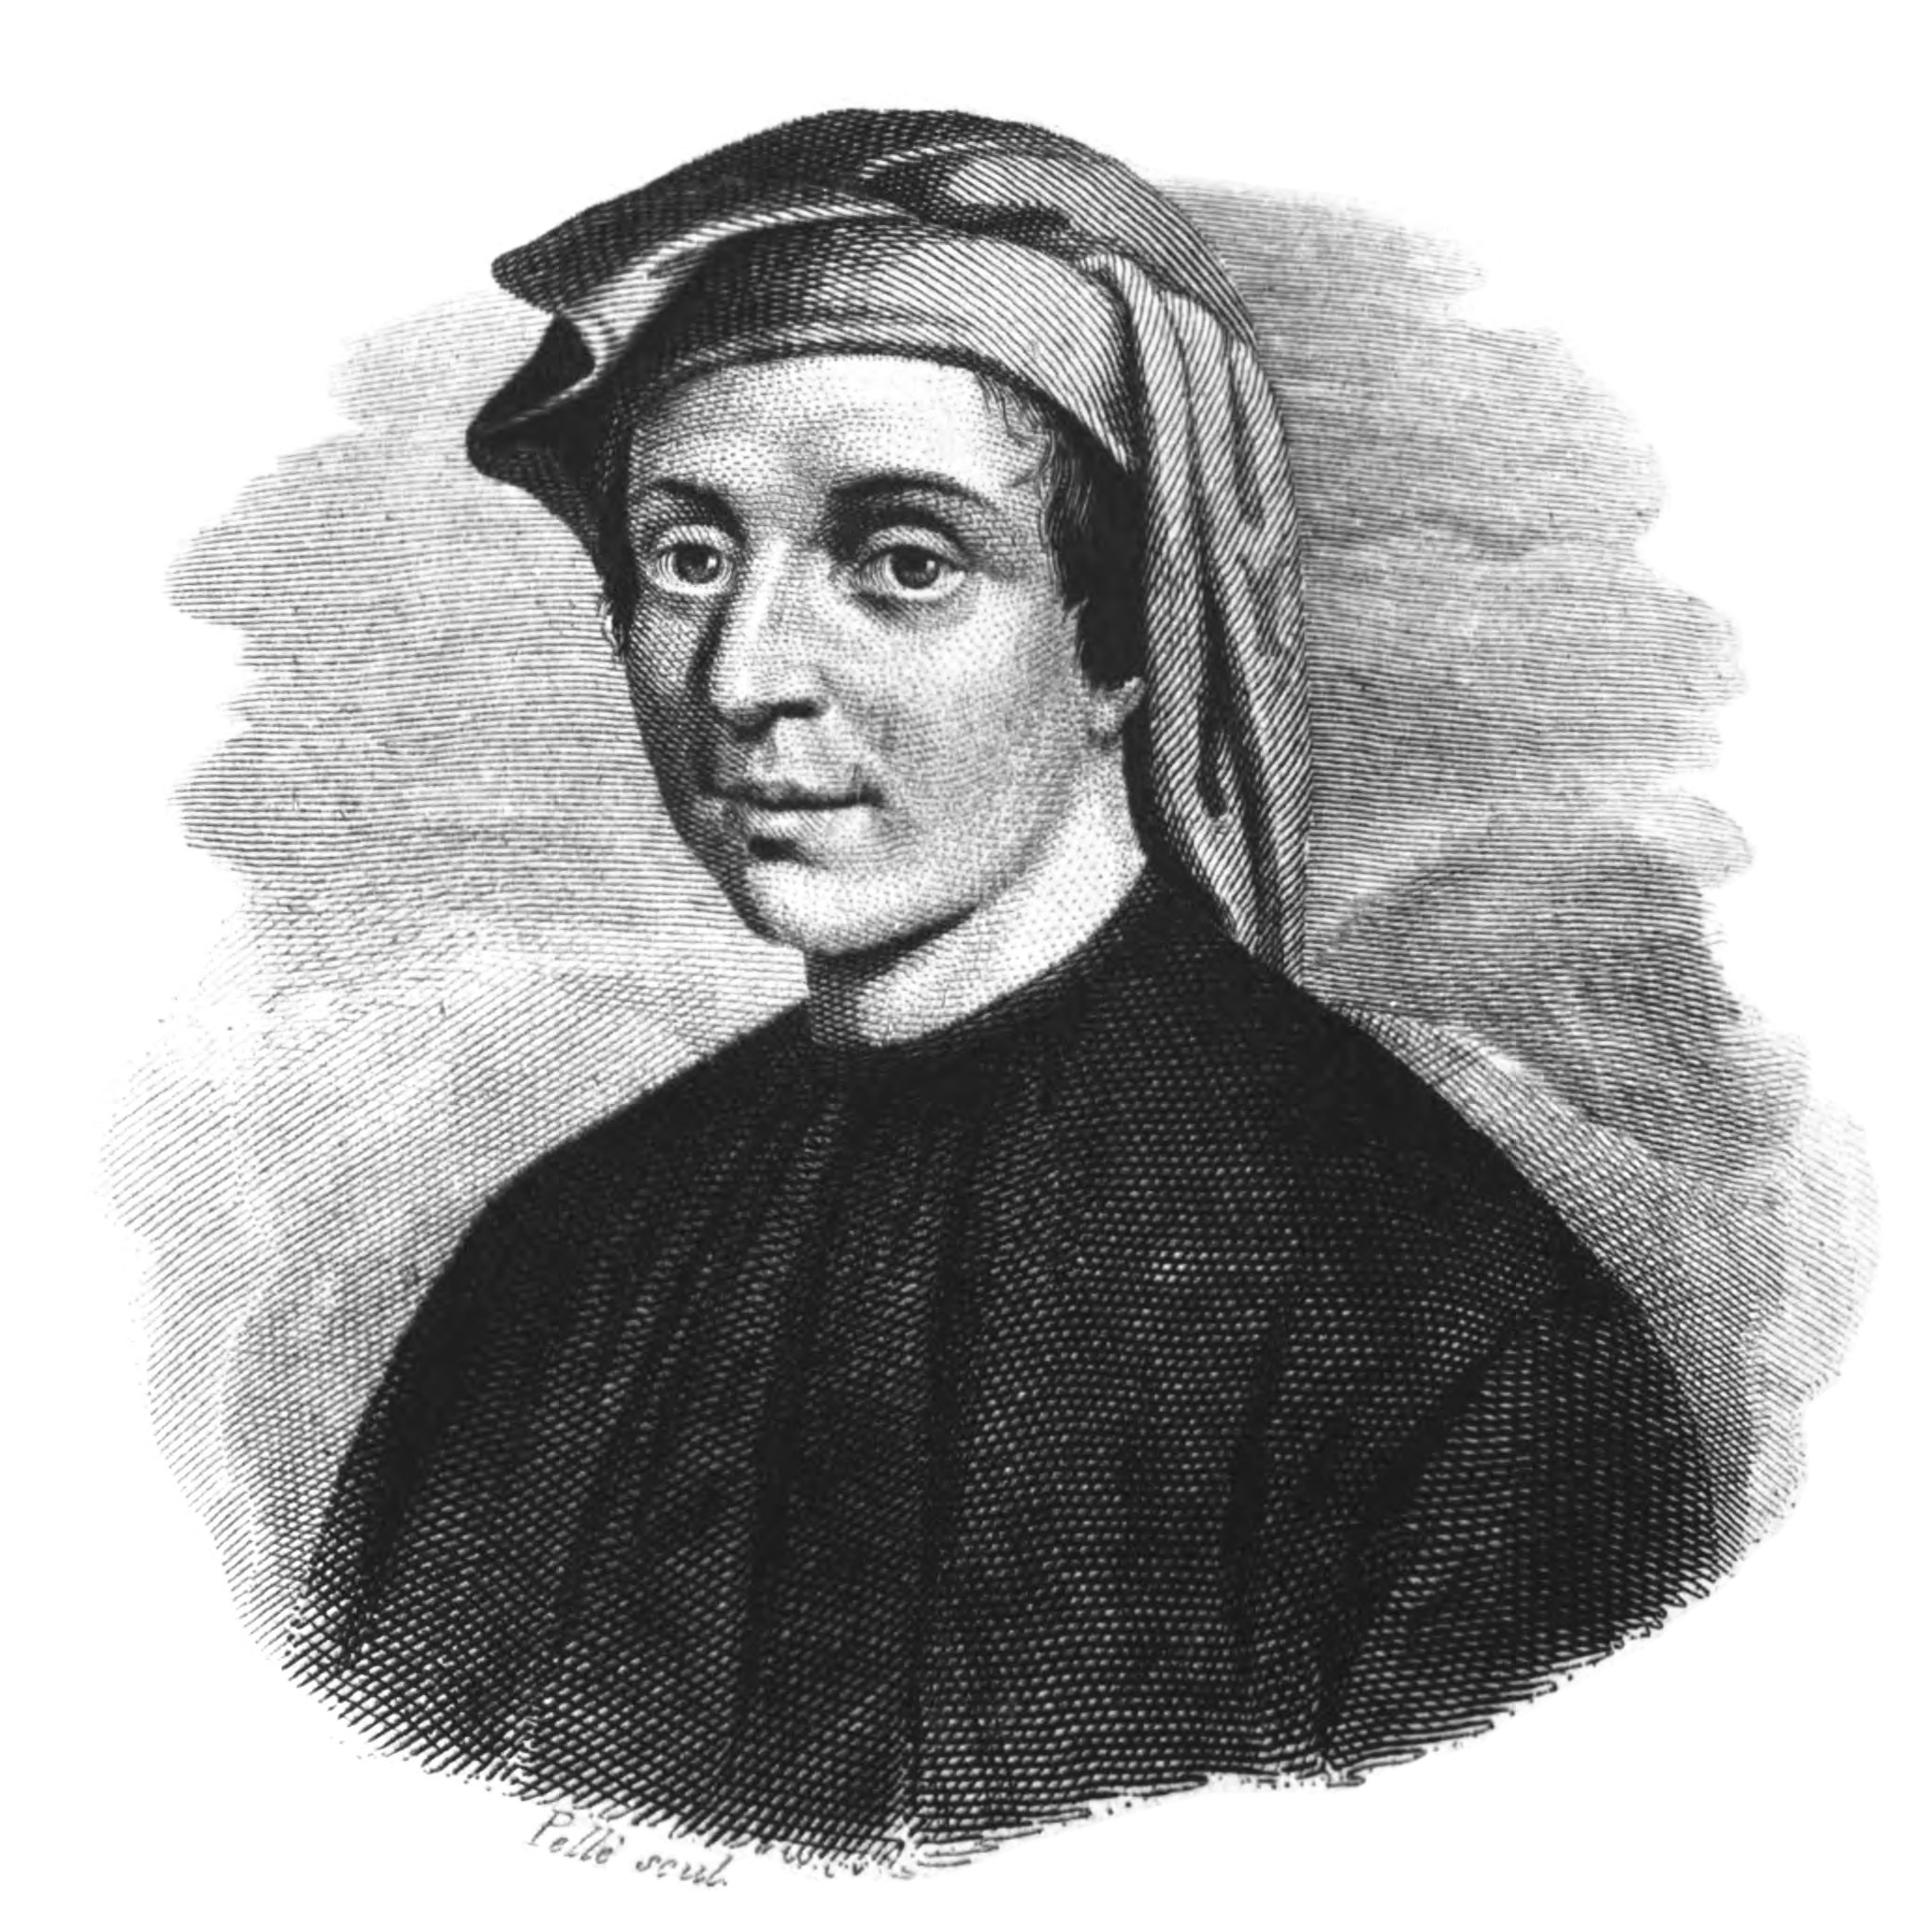
\includegraphics[width=0.38\textwidth]{Fibonacci.jpg}%
    };
  \end{tikzpicture}
  \caption[Leonardo Pisano]{\sloppy{Leonardo Pisano.}}
  \label{fig:frederick}
\end{wrapfigure}
The Euclidean parametrization of the Pythagorean triples has some further applications, but in order to get there we must make a short excursion to the city of Pisa in the 13th century, where Frederick~II reigned as the Holy Roman Emperor, and King of Sicily, Jerusalem, and Apulia. When Leonardo Pisano, more commonly known as Fibonacci, was summoned to the court of Frederick~II, he met with Master John of Palermo who challenged him with mathematical problems.

One of the challenges of Master John is stated as follows: Find a rational number $q$ such that the numbers
\begin{equation*}
  q^2-5 \qquad\text{and}\qquad q^2+5
\end{equation*}
are both squares of rational numbers. Fibonacci's investigations into this problem would eventually lead him to write his \emph{Liber Quadratorum} \cite{fibonacci1987}. The Liber Quadratorum covers topics such as Pythagorean triples, a method of generating infinitely many of them, and arithmetic progressions of squares. There were no known remaining copies of the Liber Quadratorum until a 15th century copy was rediscovered in the Biblioteca Ambrosiana in Milan, which was republished in print in 1857 by the Italian historian and mathematician Baldassarre Boncompagni Ludovisi. Today, the work available in an English translation by Laurence E.~Sigler as \emph{The Book of Squares} \cite{fibonacci1987}.

Master John's challenge is equivalently formulated as the question of finding four integers $a$, $b$, $c$, and $t$ such that
\begin{equation*}
  b^2-a^2=5t^2\qquad\text{and}\qquad c^2-b^2=5t^2.
\end{equation*}
Thus, we are looking for three squares $a^2$, $b^2$, and $c^2$ increasing in increments of $5t^2$. Thus we see that we can conveniently state the problem in terms of arithmetic triples of squares.

\begin{definition}
  An \emph{arithmetic triple of squares} is a triple $(a^2,b^2,c^2)$ consisting of integer squares such that
  \begin{equation*}
    b^2-a^2=c^2-b^2.
  \end{equation*}
  This common increment is denoted by $\Delta_{a,b,c}$, or simply $\Delta$. An arithmetic triple of squares $(a^2,b^2,c^2)$ is said to be \emph{primitive} if $\gcd(a,b,c)=1$.
\end{definition}

It follows immediately from the definition that if $(a^2,b^2,c^2)$ is a primitive arithmetic triple of squares, then $a$, $b$, and $c$ are also pairwise relatively prime.

We are thus looking for an arithmetic triple of squares, with increment of the form $\Delta:=5t^2$. In \cref{exercise:div-increment-a-p-squares} you were asked to show that the increment $\Delta$ of an arithmetic triple of squares is always divisible by $24$, which Fibonacci also reported on in Liber Quadratorum. We conclude from this observation that if $\Delta$ is of the form $5t^2$ then $\Delta$ must be a multiple of $2\cdot3\cdot 5 \cdot 24=720$.

\begin{figure}[t]
  \centering
  \resizebox{\textwidth}{!}{
    \begin{tikzpicture}
      \pgfmathdeclarefunction{dn}{1}{%
        \pgfmathparse{mod(#1,2)==1 ? #1 : int(#1/2)}%
      }

      \pgfmathtruncatemacro{\rmax}{9}
      \pgfmathtruncatemacro{\cwidth}{2*\rmax-1}
      % Loop over rows
      \foreach \row in {1,...,\rmax} {%
        
        % Vertical position
        \pgfmathsetmacro\y{(\row-1)*sqrt(3)/2}%
        
        % Columns shrink by one each row up
        \pgfmathtruncatemacro\maxc{\cwidth-(\row-1)}%
        
        \foreach \col in {1,...,\maxc} {%
          \pgfmathtruncatemacro\S{0}%
          \pgfmathtruncatemacro\J{0}%
          \pgfmathtruncatemacro\limit{\row}%
          \pgfmathloop
          \ifnum\J<\limit
            \pgfmathtruncatemacro\term{dn(\col+\J)}%
            \pgfmathtruncatemacro\S{\S+\term}%
            \pgfmathtruncatemacro\J{\J+1}%
            \repeatpgfmathloop
            \node[draw,thick,circle,minimum size=6mm,inner sep=0pt,align=center,font=\small]
              (nC\col R\row) at ({(\col-1)+(\row-1)/2},\y) {\S};%
            }%
          
        \foreach \col in {1,...,\maxc} {
          \pgfmathtruncatemacro{\ncol}{\col+1}
          \pgfmathtruncatemacro{\prow}{\row-1}
          
          \ifnum\row>1\relax
            \draw[thick] (nC\col R\row) -- (nC\col R\prow);%
            \draw[thick] (nC\col R\row) -- (nC\ncol R\prow);%
          \fi
        }%
      }%
      
      \foreach \base in {0,...,\cwidth} {%
        \pgfmathsetmacro\y{(-1)*sqrt(3)/2}
        \pgfmathtruncatemacro\pmone{\ifodd\base -1\else 1\fi}
        \pgfmathtruncatemacro\half{int((\base+1)/2)}
        \pgfmathtruncatemacro\rootval{6*\half + \pmone}
        
        \node[draw,thick,rectangle,minimum size=5.5mm,inner sep=0pt,align=center,font=\small] (b\base) at ({\base-1/2},\y) {\rootval};
        \pgfmathtruncatemacro{\leftcol}{\base}
        \pgfmathtruncatemacro{\rightcol}{\base+1}
        \ifnum\base<\cwidth
          \draw[thick] (b\base) -- (nC\rightcol R1);
        \fi
        \ifnum\base>0
          \draw[thick] (b\base) -- (nC\leftcol R1);
        \fi
      }

      % \begin{scope}[on background layer]
      %   \foreach \rowone in {1,...,\rmax}
      %   {
      %     \pgfmathtruncatemacro\maxc{\cwidth-(\rowone-1)}
      %     \foreach \colone in {1,...,\maxc}
      %     {
      %       \foreach \rowtwo in {1,...,\colone}
      %       {
      %         \pgfmathtruncatemacro\Sone{0}%
      %         \pgfmathtruncatemacro\Jone{0}%
      %         \pgfmathtruncatemacro\limitone{\rowone}%
      %         \pgfmathloop
      %         \ifnum\Jone<\limitone
      %           \pgfmathtruncatemacro\termone{dn(\colone+\Jone)}%
      %           \pgfmathtruncatemacro\Sone{\Sone+\termone}%
      %           \pgfmathtruncatemacro\Jone{\Jone+1}%
      %           \repeatpgfmathloop
                
      %         \pgfmathtruncatemacro\coltwo{\colone-\rowtwo}
      %         \pgfmathtruncatemacro\maxctwo{\cwidth-(\rowtwo-1)}
      %         \pgfmathtruncatemacro\Stwo{0}%
      %         \pgfmathtruncatemacro\Jtwo{0}%
      %         \pgfmathtruncatemacro\limittwo{\rowtwo}%
      %         \pgfmathloop
      %         \ifnum\Jtwo<\limittwo
      %           \pgfmathtruncatemacro\termtwo{dn(\coltwo+\Jtwo)}%
      %           \pgfmathtruncatemacro\Stwo{\Stwo+\termtwo}%
      %           \pgfmathtruncatemacro\Jtwo{\Jtwo+1}%
      %           \repeatpgfmathloop
                
      %         \ifnum\Sone=\Stwo\relax
      %           % fill both nodes
      %           \fill[YellowOrange] (nC\colone R\rowone) circle (3mm);
      %           \fill[CornflowerBlue] (nC\coltwo R\rowtwo) circle (3mm);
      %         \fi
      %       }
      %     }
      %   }
      % \end{scope}
      
      \begin{scope}[on background layer]
        \fill[CornflowerBlue] (nC1R1) circle (3mm);
        \fill[YellowOrange] (nC2R1) circle (3mm);
        \fill[CornflowerBlue] (nC3R2) circle (3mm);
        \fill[YellowOrange] (nC5R1) circle (3mm);
        \fill[CornflowerBlue] (nC3R3) circle (3mm);
        \fill[YellowOrange] (nC6R2) circle (3mm);
        \fill[CornflowerBlue] (nC6R3) circle (3mm);
        \fill[YellowOrange] (nC9R2) circle (3mm);
        \fill[CornflowerBlue] (nC1R9) circle (3mm);
        \fill[YellowOrange] (nC10R4) circle (3mm);
        \fill[CornflowerBlue] (nC8R5) circle (3mm);
        \fill[YellowOrange] (nC13R3) circle (3mm);
        \fill[CornflowerBlue] (nC11R3) circle (3mm);
        \fill[YellowOrange] (nC14R3) circle (3mm);
      \end{scope}
    \end{tikzpicture}
  }
  \caption[Differences of squares congruent to $1$ modulo $24$]{\label{figure:quotients-of-differences-of-squares}The numbers in squares at the base of the grid are the numbers of the form $6m\pm 1$, which correspond exactly to all the numbers $n$ such that $n^2-1$ is divisible by $24$. If $x$ and $y$ are two numbers in squares at the base of the grid, then the number $k$ at the apex of the triangle spanned by $x$ and $y$ satisfies $y^2-x^2=k\cdot 24$. For each primitive arithmetic triple $(x^2,y^2,z^2)$ of squares, the apex of the triangle spanned by $x$ and $y$ is marked in blue, and the apex of the triangle spanned by $y$ and $z$ is marked in orange.
  }
\end{figure}

The fact that the common increment in an arithmetic triple of squares is always a multiple of $24$ implies that primitive arithmetic triples of squares consist entirely of integers of the form $(6m\pm 1)^2$. Any such square exceeds a multiple of $24$ by one. This significantly reduces the search space for arithmetic triples of squares. If $a_n$ is the $n$th positive integer of the form $(6k\pm 1)^2$, then
\begin{equation*}
  d_n:=\frac{a_{n+1}-a_n}{24}=
  \begin{cases}
    n & \text{if $n$ is odd,}\\
    n/2 & \text{if $n$ is even.}
  \end{cases}
\end{equation*}
In order to determine the number of units of $24$ in the difference between two arbitrary numbers of the form $(6m\pm 1)^2$, we simply sum the numbers $d_n$: We define
\begin{equation*}
  s_{n,m}:=\sum_{i=0}^md_{n+i}=\frac{a_{n+m+1}-a_n}{24}.
\end{equation*}
Alternatively, the numbers $s_{n,m}$ are determined by the recursive rule $s_{n,m}=s_{n+1,m-1}+s_{n,m-1}-s_{n+1,m-2}$.
The numbers $s_{n,m}$ are displayed in \cref{figure:quotients-of-differences-of-squares}, from which we determine that:
    \begin{align*}
      5^2-1^2 & = 7^2-5^2 & & = 1\cdot 24, \\
      13^2 - 7^2 & = 17^2 - 13^2 & & = 5\cdot 24, \\
      17^2 - 7^2 & = 23^2 - 17^2 & & = 10\cdot 24, \\
      25^2 - 17^2 & = 31^2 - 25^2 & & = 14\cdot 24, \\ 
      29^2 - 1^2 & = 41^2 - 29^2 & & = 35\cdot 24, \\
      37^2 - 23^2 & = 47^2 - 37^2 & & = 35\cdot 24, \\
      41^2 - 31^2 & = 49^2 - 41^2 & & = 30\cdot 24.
    \end{align*}
The solution to Master John's problem to Fibonacci, which Fibonacci reported in Proposition 17 of \emph{Liber Quadratorum}, thus corresponds to the last listed arithmetic triple of squares, which gives
\begin{equation*}
  \left(\frac{41}{12}\right)^2-\left(\frac{31}{12}\right)^2=\left(\frac{49}{12}\right)^2-\left(\frac{41}{12}\right)^2=5.
\end{equation*}

% \begin{proposition}
%   If $a$, $b$, and $c$ are integers such that
%   \begin{equation*}
%     \Delta:=b^2-a^2=c^2-b^2,
%   \end{equation*}
%   then $24\mid \Delta$.
% \end{proposition}

% \begin{proof}
%   We will prove separately that $\Delta$ is of the form $8k$ and of the form $3k$. Recall that even squares are of the form $4k$, while odd squares are of the form $8k+1$, implying that differences of squares cannot be of the form $4k+2$. Since both $\Delta$ and $2\Delta$ occur as the difference of squares, where $2\Delta=c^2-a^2$, it follows that $\Delta$ must be of the form $4k$.

%   It follows that $a^2$, $b^2$, and $c^2$ are either all even or all odd. By dividing out any common factors of $a^2$, $b^2$, and $c^2$ we may assume that they are all odd, which implies that $\Delta$ is a multiple of $8$.

%   To see that $\Delta$ is a multiple of $3$, recall that all odd squares are of the form $36k+9$ or $12k+1$, so that differences of odd squares are of the form $12k$, $12k+8$, or $12k+10$. Since $\Delta=b^2-a^2$ can only be of the form $12k+8$ if $b\equiv \pm{1}\pmod{6}$ and $a\equiv 3\pmod 6$, there cannot be a square $c^2$ such that $c^2-b^2$ is also of the form $12k+8$. Likewise we rule out $12k+10$ from the possible options for $\Delta$. Thus, we conclude that $\Delta$ is a multiple of $12$, and in particular it is a multiple of $3$.
% \end{proof}

Arithmetic triples of squares are closely related to Pythagorean triples. Given an arithmetic triple of squares $(a^2,b^2,c^2)$, we can write $b^2$ as a sum of two squares written in terms of $a$ and $c$. The crucial identity that leads to the construction of a Pythagorean triple using the integers $a$, $b$, and $c$ is
\begin{equation*}
  c^2+a^2=2b^2.
\end{equation*}
Using this identity, we see that
\begin{equation*}
  \frac{(c-a)^2}{4}+\frac{(c+a)^2}{4}= \frac{c^2-2ac+a^2}{4}+\frac{c^2+2ac+a^2}{4} = \frac{c^2+ a^2}{2} = b^2.
\end{equation*}
Thus, if $(a^2,b^2,c^2)$ is an arithmetic progression of squares, then the integers
\begin{equation*}
  x := \frac{c-a}{2},\qquad y:= \frac{c+a}{2},\qquad\text{and}\qquad z:= b
\end{equation*}
determine a Pythagorean triple $(x,y,z)$. Conversely, if $(x,y,z)$ is a Pythagorean triple, then we define
\begin{equation*}
  a := |y-x|, \qquad b := z,\qquad\text{and}\qquad c:= y+x,
\end{equation*}
so that $(a^2,b^2,c^2)$ is easily seen to be an arithmetic triple of squares. Here, we defined $a$ to be the \emph{distance} between $y$ and $x$ in order to ensure that $a$ is positive. The common increment in this arithmetic triple is given by
\begin{equation*}
  z^2-(y-x)^2=2xy,
\end{equation*}
which is four times the area of the Pythagorean triangle described by the Pythagorean triple $(x,y,z)$.
The operations thus described create the following correspondence between some of the most familiar arithmetic triples of squares and Pythagorean triples:
\begin{align*}
  (1^2,5^2,7^2)   & \bimapsto (3,4,5), \\
  (7^2,13^2,17^2) & \bimapsto (5,12,13), \\
  (1^2,29^2,41^2) & \bimapsto (21,20,29), \\
  (7^2,17^2,23^2) & \bimapsto (15,8,17).
\end{align*}
The fact that these operations mapping arithmetic triples of squares to Pythagorean triples and back are mutually inverse to each other is easily verified by a few quick computations, which we leave to the reader. Thus, we have established:

\begin{theorem}\label{theorem:correspondence-arithmetic-triples-squares}
  Arithmetic triples $(a^2,b^2,c^2)$ of squares are in bijective correspondence with Pythagorean triples $(x,y,z)$, so that primitive arithmetic triples of squares correspond to primitive Pythagorean triples.
\end{theorem}

\begin{proof}
  We only prove that $(a^2,b^2,c^2)$ is a primitive arithmetic triple of squares if and only if the Pythagorean triple
  \begin{equation*}
    \left(\tfrac{c-a}{2},\tfrac{c+a}{2},b\right)
  \end{equation*}
  is primitive.

  For the forward direction, assume that $\gcd(a,b,c)=1$. To see that $(c-a)/2$ and $(c+a)/2$ are relatively prime, it suffices to show that any common divisor $d$ of $c-a$ and $c+a$ is a divisor of $2$. Indeed, if $d$ is a common divisor of $c-a$ and $c+a$, then it is also a common divisor of $2a=(c+a)-(c-a)$ and $2c=(c+a)+(c-a)$. Since $a$ and $c$ are relatively prime, it follows that $d$ is a divisor of $2$.

  Likewise, to show that $(c-a)/2$ and $b$ are relatively prime, we note that since $b$ is odd it suffices to show that $c-a$ and $b$ are relatively prime, which is only the case if $(c-a)^2$ and $b^2$ are relatively prime. This follows from
  \begin{equation*}
    (c-a)^2=c^2+a^2-2ac=2b^2-2ac,
  \end{equation*}
  since any common divisor of $(c-a)^2$ and $b^2$ is also a common divisor of $b^2$ and $2ac$, which are relatively prime by assumption. The proof that $(c+a)/2$ and $b$ are relatively prime is similar. 

  For the reverse direction, assume that
  \begin{equation*}
    \left(\tfrac{c-a}{2},\tfrac{c+a}{2},b\right)
  \end{equation*}
  is a primitive Pythagorean triple, so that $b$ is odd, and thus $b$, $(c-a)/2$, and $(c+a)/2$ are all pairwise relatively prime. Then any common divisor $d$ of $a$ and $c$ is also a common divisor of $(c-a)/2$ and $(c+a)/2$, so that $a$ and $c$ are seen to be relatively prime.

  We will prove that $(x,y,z)$ is a primitive Pythagorean triple if and only if
  \begin{equation*}
    ((y-x)^2,z^2,(y+x)^2)
  \end{equation*}
  is a primitive arithmetic triple of squares. By Euclid's parametrization of Pythagorean triples, it suffices to show that for any two
\end{proof}

The previous theorem raises an interesting point. Since the primitive Pythagorean triples are precisely described by Euclid's parametrization, there must similarly be a parametrization of the arithmetic triples of squares.

\begin{corollary}
  For any primitive arithmetic triple of squares $(a^2,b^2,c^2)$, we can uniquely determine two relatively prime positive integers $s<t$ of opposite parity such that
  \begin{equation*}
    a=2st-t^2+s^2,\qquad b=t^2+s^2,\qquad\text{and}\qquad c=2st+t^2-s^2
  \end{equation*}
  with common difference $d= 2st(t-s)^2$.
\end{corollary}

\begin{exercises}
  \exercise \emph{Bhaskara's proof of the Pythagorean Theorem.} Use the following diagram to give a proof of the \crefnamed{theorem:pythagorean-theorem}{Pythagorean Theorem}:
  \begin{equation*}
    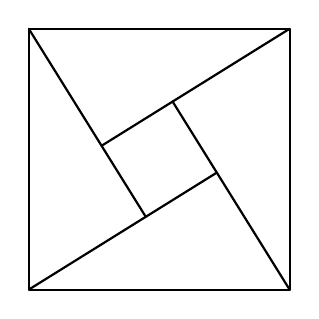
\begin{tikzpicture}[scale=.0625,thick,line join=round,line cap=round]
      \pgfmathsetmacro{\myangle}{atan(28/45)}
      \draw (0,0) rectangle (53,53);
      \foreach \k/\x/\y in {0/0/0, 1/53/0, 2/53/53, 3/0/53}
      \draw (\x,\y) -- ++({\myangle + 90*\k}:45);
    \end{tikzpicture}
  \end{equation*}
  \exercise \label{exercise:addition-laws-sin-cos}
  \exercise \label{exercise:brahmagupta-fibonacci-identity}\emph{The Brahmagupta--Fibonacci identity.} Show that
  \begin{equation*}
    (a^2+b^2)(c^2+d^2)=(ac\pm bd)^2 + (ad\mp bc)^2.
  \end{equation*}
  Conclude that if $m$ and $n$ are two integers that can be written as the sum of two squares, then their product $mn$ can also be written as the sum of two squares.
  \exercise \label{exercise:divisibility-legs-pythagorean-triples}Consider a primitive Pythagorean triple $(x,y,z)$.
  \begin{subexenum}
  \item Prove that exactly one of $x$, $y$, and $z$ is divisible by $3$.
  \item Prove that exactly one of $x$, $y$, and $z$ is divisible by $5$.
  \item Find all Pythagorean triples $(x,y,z)$ in which $x=30$ or $y=30$. Can any of them be primitive?
    % (30,16,34),
    % (30,40,50),
    % (30,72,78),
    % (30,224,226)
  \item Find all relatively prime positive integers $x$ and $z$ such that
    \begin{equation*}
      x^2+60^2=z^2,
    \end{equation*}
    showing that the components divisible by $3$, $4$, or $5$ might all coincide.
    % (11,60,61),
    % (91,60,109),
    % (221,60,229),
    % (899,60,901).
  \end{subexenum}
  \exercise Show that for every positive integer $y$ divisible by $4$, there is a primitive Pythagorean triple of the form $(x,y,z)$.
  \exercise Show that every odd positive integer $x\geq 3$ can be written in the form $s^2-t^2$, so that there is a primitive Pythagorean triple of the form $(x,y,z)$.
  \exercise Define
  \begin{align*}
    x_n & := F_n F_{n+1}+(-1)^n, \\
    y_n & := 2F_nF_{n+1}, \\
    z_n & := F_{n}^2+F_{n+1}^2,
  \end{align*}
  where $F_k$ is the $k$th Fibonacci number. Show that $(x_n,y_n,z_n)$ is a Pythagorean triple for each $n$.
  \exercise Let
  \begin{align*}
    a_n & := F_{n}F_{n+1}- (-1)^n, \\
    b_n & := F_{n}^2 + F_{n+1}^2, \\
    c_n & := 3F_{n}F_{n+1}+(-1)^{n}.
  \end{align*}
  be defined as in \cref{exercise:arithmetic-progression-fibonacci}, so that $(a_n^2,b_n^2,c_n^2)$ is an arithmetic triple of squares. Show that
  \begin{equation*}
    \gcd(a_n,b_n,c_n)=
    \begin{cases}
      2 & \text{if $n\equiv 1\pmod{3}$,}\\
      1 & \text{otherwise.}
    \end{cases}
  \end{equation*}
    \exercise Consider three squares $a^2$, $b^2$, and $c^2$ in an arithmetic progression in increasing order.
  \begin{subexenum}
  \item Show that at least one of
    \begin{equation*}
      c-b,~c-a,~\text{and}~b-a
    \end{equation*}
    is divisible by $3$.
  \item Show that at least one of
    \begin{equation*}
      c-b,~c-a,~\text{and}~b-a
    \end{equation*}
    is divisible by $4$.
  \item Show that at least one of
    \begin{equation*}
      b~\text{and}~c-a
    \end{equation*}
    is divisible by $5$.
  \item Find all arithmetic progressions $(a^2,b^2,c^2)$ such that $c-a=60$, where only $a$ is allowed to be negative. Are there any such triples with $\gcd(a,b,c)=1$?
    % (-14,34,46),
    % (10,50,70),
    % (42,78,102),
    % (194,226,254)
  \item Find all \emph{primitive} arithmetic progressions $(a^2,b^2,c^2)$ such that $c-a=120$, where only $a$ is allowed to be negative. Hint: There are four such triples.
    % (−49,61,71)
    % (31,109,151)
    % (161,229,281)
    % (839,901,959)
  \end{subexenum}
  \exercise Find all solutions to the equation $x^2-2y^2=1$.
  \exercise \emph{Master Theodore's problem for Leonardo Pisano \cite[Proposition 24]{fibonacci1987}.} Find three positive integers $x$, $y$, and $z$ such that the numbers
  \begin{equation*}
    x+y+z+x^2,\qquad x+y+z+x^2+y^2,\qquad\text{and}\qquad x+y+z+x^2+y^2+z^2
  \end{equation*}
  are all squares.
  \exercise Find three distinct triangular numbers in an arithmetic progression.
  \exercise Find three distinct tetrahedral numbers, that is, numbers of the form $\binom{n+2}{3}$, in an arithmetic progression.
\end{exercises}

%%% Local Variables:
%%% mode: latex
%%% TeX-master: "elementary-number-theory"
%%% End:
